%----------------------------------------------------------------------
%	DIRC TECHNOLOGY CHAPTER
%----------------------------------------------------------------------
\label{ch:components}
The validation of the key components of the DIRC for an EIC discussed in Chapter \ref{ch:eicdirc} is vital to show that the GEANT4 simulation package produces results expected for the real detector. However, due to budget restraints it was not possible to build or otherwise procure a full scale prototype of the envisioned EIC DIRC discussed in Chapter \ref{ch:eicdirc}. As a conservative estimate of the cost of a simple prototype: one radiator bar is \$20k, a prism expansion volume is \$30k, a 3-layer lens is \$10k, and an array of 24 (4x6) sensors is \$200k. On top of this, the cost of a test beam run would be roughly \$10k for travel and expenses.  This roughly \$300k expense for one prototype and test beam is highly impractical given that the budget for all detector work for the EIC R\&D effort (RICH, Time-of-Flight, simulation studies, calorimetry, etc) is only \$1M/year. Instead a series of test bench measurements have been made to validate simulated performance of the new 3-layer lens design, study the radiation hardness of the NLaK33 material, and evaluate the performance of MCP-PMTs in high magnetic field environments. A synergistic test beam effort with the PANDA Barrel DIRC group was also performed at CERN in 2015, but will be discussed in greater detail in Chapter \ref{ch:analysis}.

%----------------------------------------------------------------------
%	3-LAYER LENS OPTICS SECTION
%----------------------------------------------------------------------
\section{Optical Properties of 3-Layer Lens}
\begin{figure}[!htb]
	\centering
	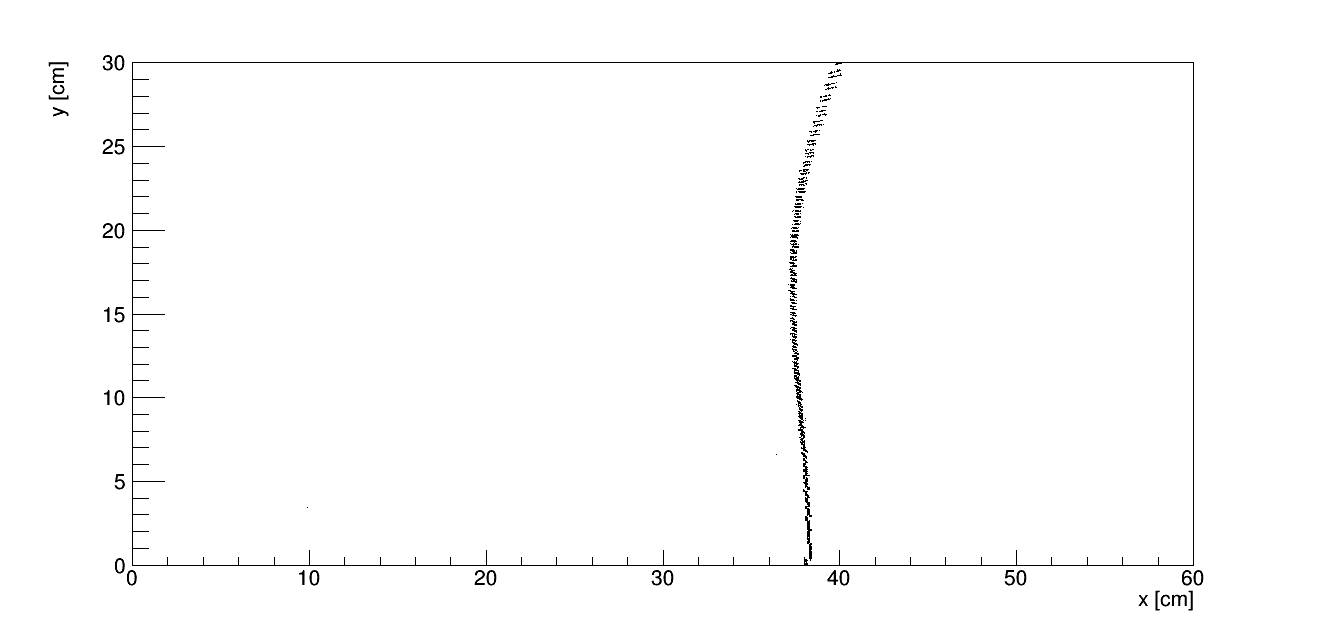
\includegraphics[width=\textwidth]{2D_plane.png}
	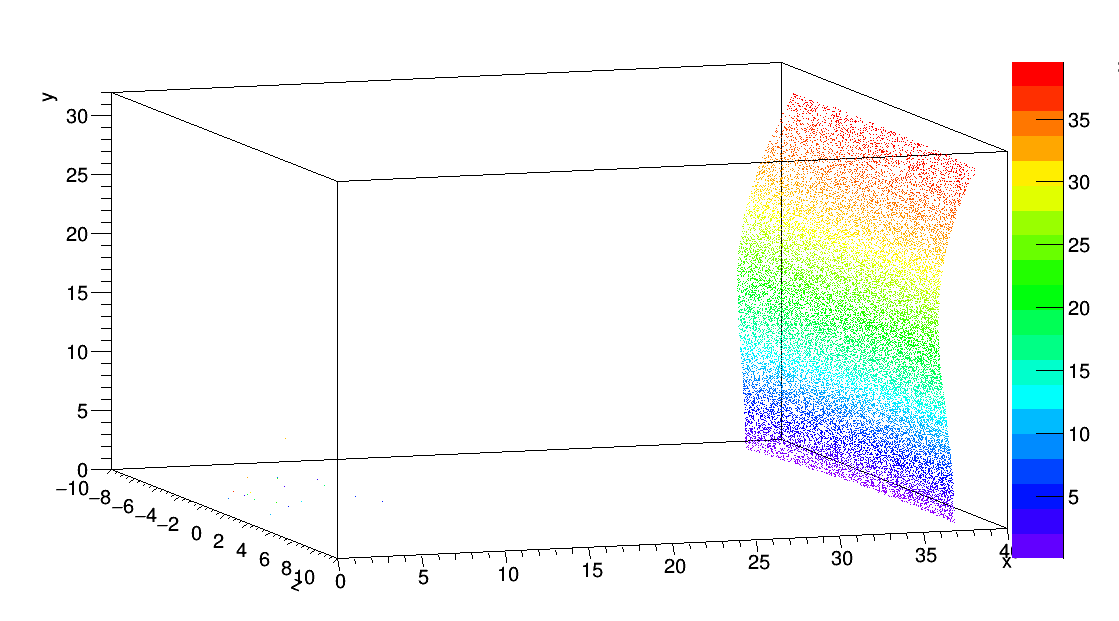
\includegraphics[width=\textwidth]{3D_plane_angle.png}
	\caption{Simulation of the 3-layer lens focal plane with all photons confined to a single plane (top) and the full 3D focal plane (bottom). The color scale corresponds to the initial angle (in degrees) between the laser beams and the lens face. The 3D plane has been constrained to the y/z dimensions of the current expansion volume for the EIC DIRC. The ``beams" of photons in the simulation were centered around the center of the lens with a separation of 2 mm.}
	\label{fig:focalplane_sim}
\end{figure}
\begin{figure}[!htb]
	\centering
	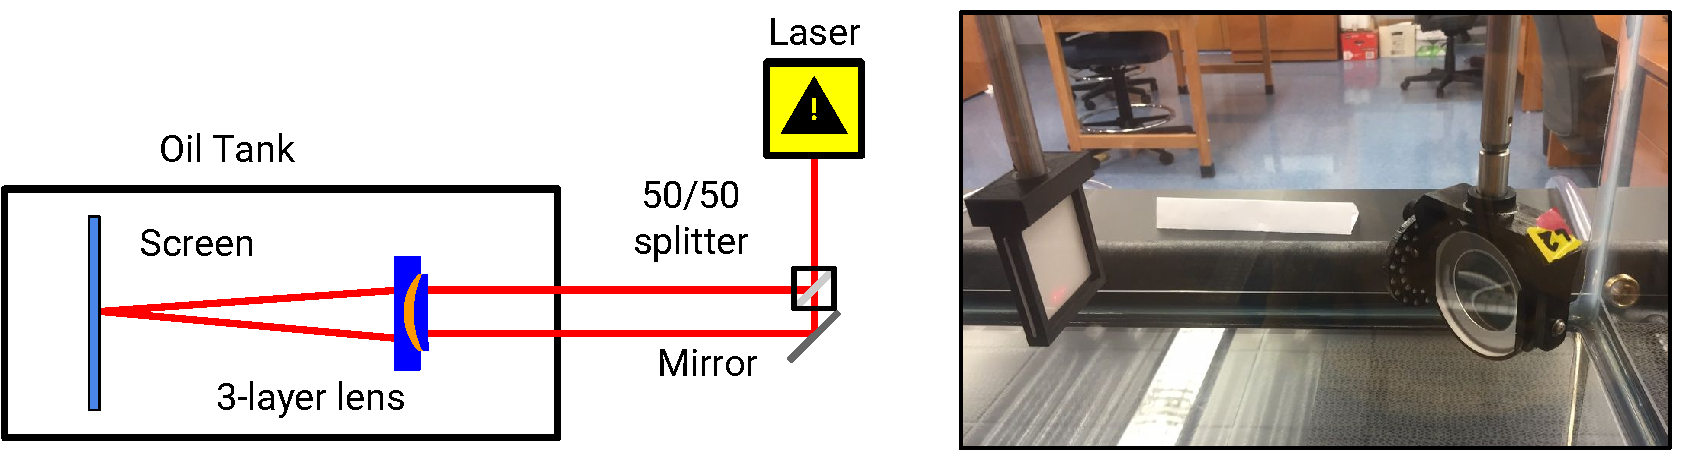
\includegraphics[width=\textwidth]{lens_setup_schematic.pdf}
	\caption{Schematic drawing of the setup built at Old Dominion University for testing the optical properties of the 3-layer lens design (left), and a closeup view of the lens and screen inside the actual setup (right).}
	\label{fig:ODU_setup}
\end{figure}

\begin{figure}[!htb]
	\centering
	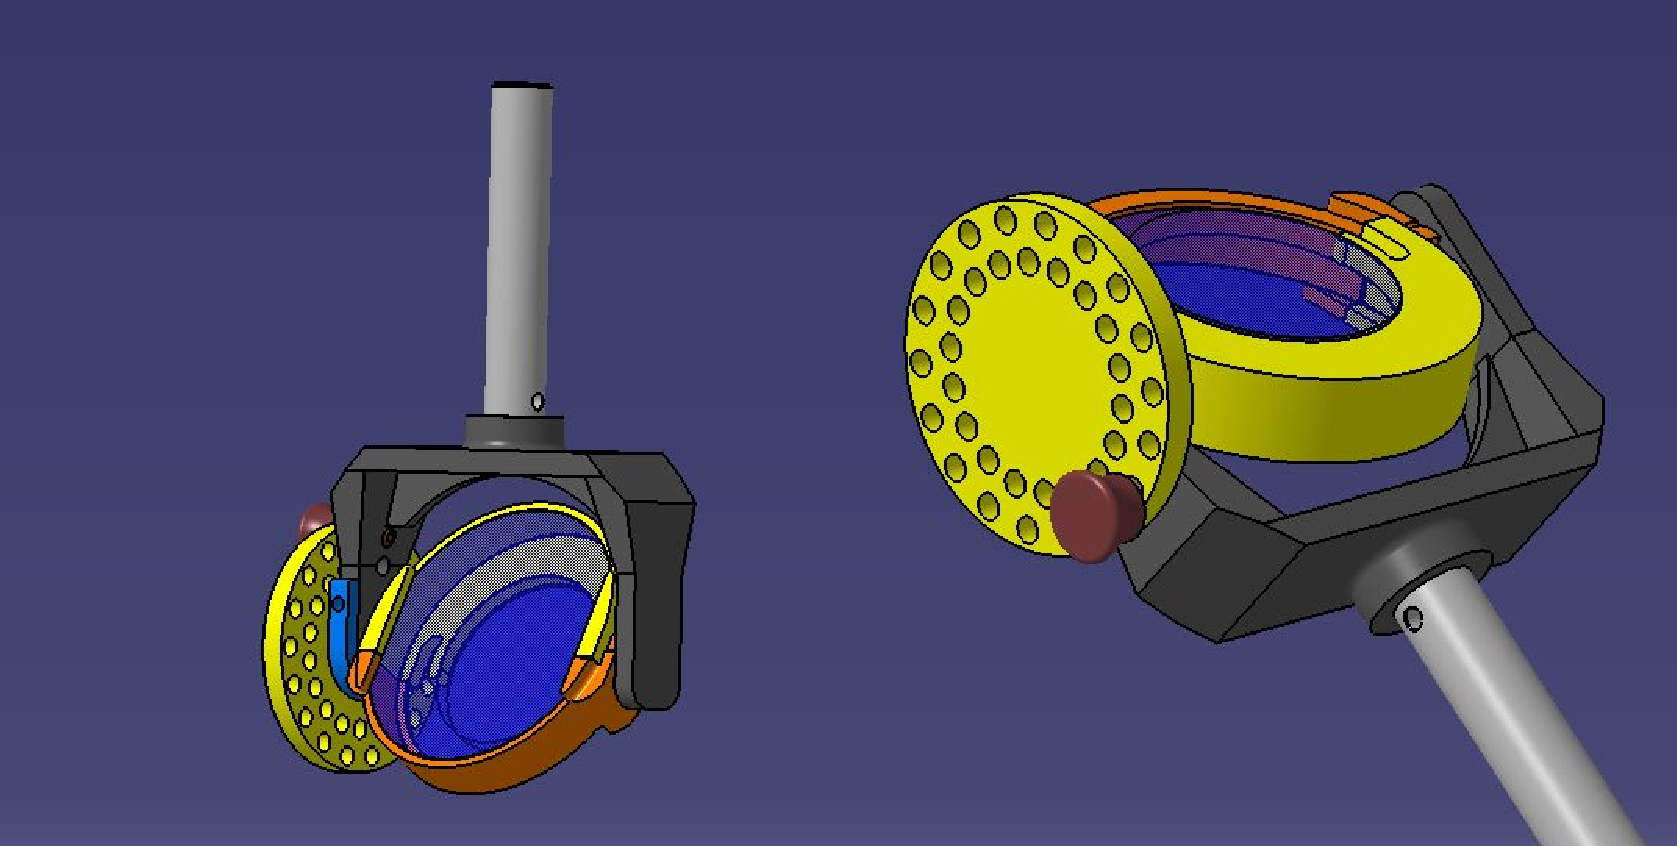
\includegraphics[width=\textwidth]{lens_holder.pdf}
	\caption{CAD drawing of 3-layer lens holder which allows precision rotation in two orthogonal, allowing the full 3D focal plane to be mapped.}
	\label{fig:lens_holder}
\end{figure}

\begin{figure}[!htb]
	\centering
	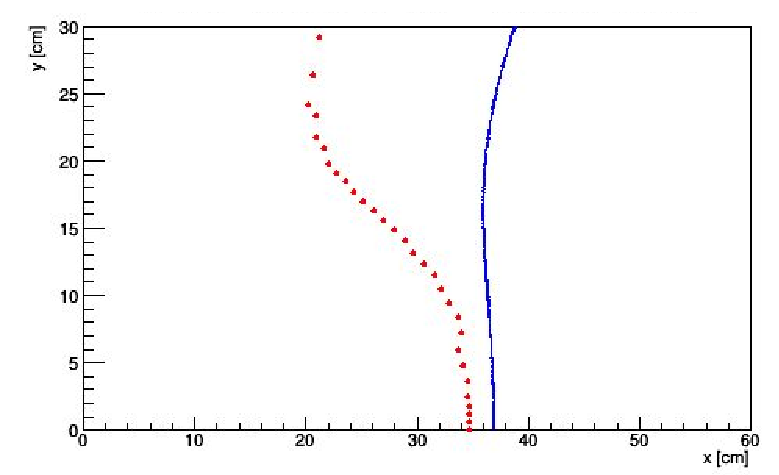
\includegraphics[width=\textwidth]{focalplane_initial.pdf}
	\caption{Initial measurement of the 3-layer lens focal plane using the upgraded green laser (red dots) compared to simulation (blue line). Note that this figure is for illustrative purposes only. The measurement techniques used to measure the focal plane were changed to match the simulation, shown in Figure \ref{fig:focalplane_corrections}.}
	\label{fig:focalplane_initial}
\end{figure}

\begin{figure}[!htb]
	\centering
	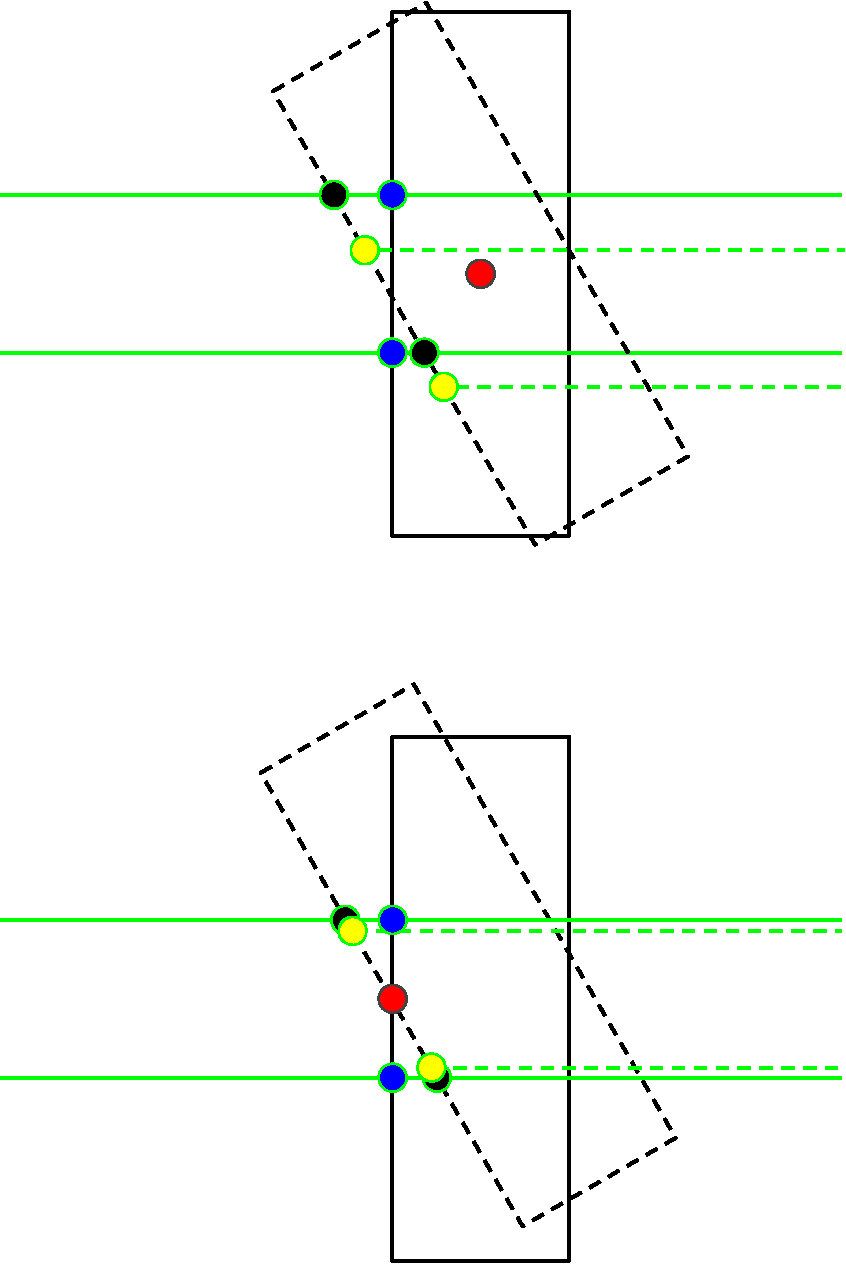
\includegraphics[width=0.43\textwidth]{lens_rotation_point.pdf}
	\caption{Illustration of the discrepancy between beam positions in data (black) and simulation (yellow) in relation to the original beam positions (blue) for a given rotation point (red) at the center (top) of the lens, or at the edge (bottom) of the lens. }
	\label{fig:lens_rotation_point}
\end{figure}

\begin{figure}[!htb]
	\centering
	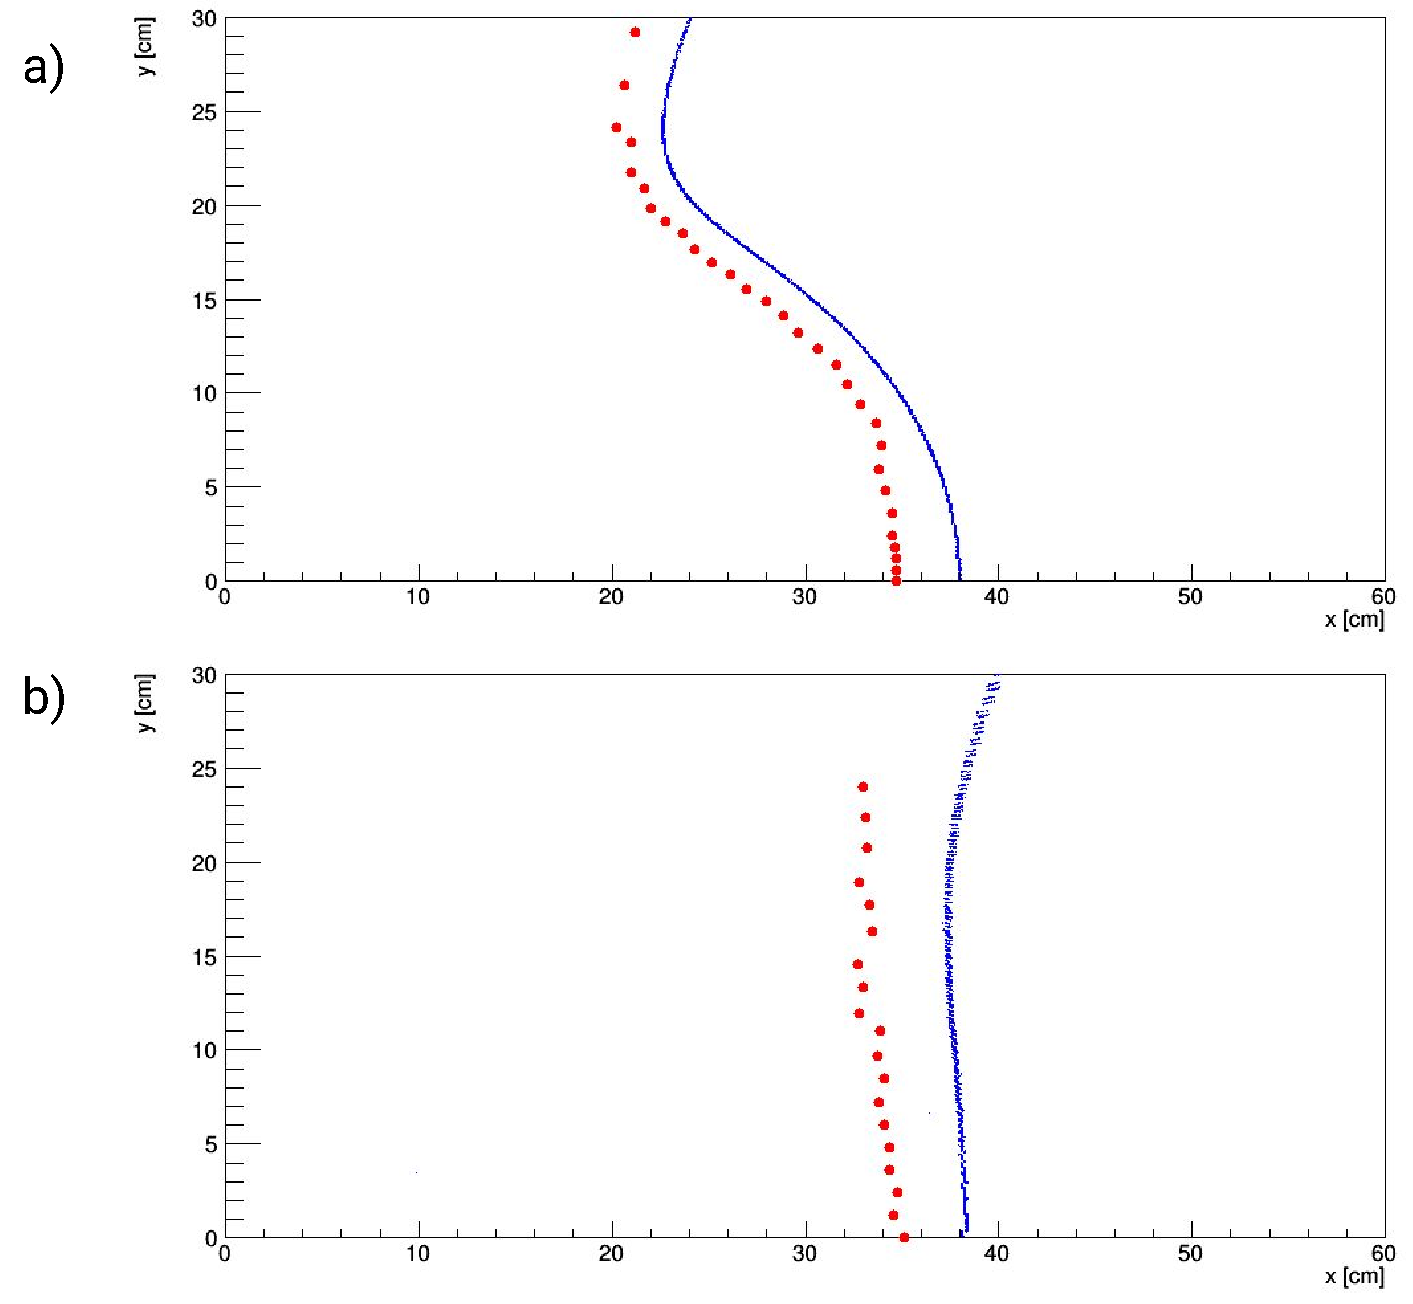
\includegraphics[width=\textwidth]{focalplane_corrections.pdf}
	\caption{Initial measurement of the 3-layer lens focal plane compared to a rotation corrected simulation (a), and a second measurement with a tighter (2 mm) beam configuration and a modified lens holder (b).}
	\label{fig:focalplane_corrections}
\end{figure}

The purpose of the 3-layer lens design is to provide a mostly flat, uniform focal plane to follow the face of the detector plane. Doing so provides better resolution and hence better performance compared to standard focusing options, which typically have very curved, hyperbolic focal planes. A GEANT4 simulation of the nominal (top) and full 3D focal plane (bottom) of the lens are shown in Figure \ref{fig:focalplane_sim}. The 3D plane has been limited to the size of the detector plane anticipated for the EIC DIRC, and the color scale indicates the angle at which photons intersected the front face of the lens. Because only the total focal length is of interest the depth of the expansion volume was limited so that no bounces occurred.

To measure the shape of the focal plane a setup was designed and built, shown in Figure \ref{fig:ODU_setup}, at Old Dominion University in which a laser shines through a 50/50 beam splitter and a mirror to make two parallel beams. Initially the beams were separated by 5 mm, but gradually the distance was reduced to 1 mm in order to attempt to avoid non-uniform aberrations due to small misalignments as much as possible. The beams then pass through a $30\times40\times60\unit{cm}^3$ glass container filled with Britol 9NF White Mineral Oil \cite{BritolOil} with a refractive index similar to that of fused silica to simulate the behavior of light passing from bar to lens to expansion volume. The beams are focused through the 3-layer lens prototype, being held in a specially designed holder that allows the lens to be rotated in two planes (Figure \ref{fig:lens_holder}). Finally the beams are focused onto a plastic screen inside the tank that is attached to a track and allowed to slide freely. Due to the relatively low resolution of the human eye and the finite size of the beams the exact point of focus was difficult to measure, so an averaging method was used in which the median of the two points where the beams seem to converge and diverge was taken to be the focal point (see Figure \ref{fig:laser_crossing}). This lead to much more accurate and reproducible results.

\begin{figure}[!htb]
	\centering
	
\includegraphics[width=\textwidth]{laser_crossing.pdf}
	\caption{Illustration of two crossing laser beams (green) with finite size. During measurements all the space between the two red circles was perceived as a single point. To counteract this effect the focal point was taken as the average point between where the beams first seem to come together and where they seem to again separate.}
	\label{fig:laser_crossing}
\end{figure}

Measurements were initially taken with a 632 nm red helium-neon laser, but the beam spot was too large and very distorted. A 530 nm wavelength green laser with a 1 mm beam spot was then purchased as a replacement. Initial results with a 5 mm beam separation are shown in Figure \ref{fig:focalplane_initial}. Obviously there is a large discrepancy in both position and shape of the measured and simulated focal plane. This was rectified by discovering that in the simulation it was assumed that the two beams were entering the lens at fixed points on the lens' face regardless of lens rotation, where as in the experiment the rotation of the lens about it's center causes the beams to shift with respect to the lens face. When rotating at the edge of the lens closest to the laser rather than through the center this difference is negligible, as illustrated in Figure \ref{fig:lens_rotation_point}.

A correction was implemented in the GEANT4 simulation to account for the shift of the beam spot during rotation, the results of which can be seen in Figure \ref{fig:focalplane_corrections}a. The beams have since been brought to a 2 mm separation to reduce effects of aberration and a second lens holder was 3D printed to allow for rotation about the edge of the lens. A new round of data was taken and results are shown in Figure \ref{fig:focalplane_corrections}b. This change vastly improved the results of both the simulation from the first measurement and the results of the second, showing that the simulation indeed reproduces very nicely the shape of the focal plane, although the position is still roughly 3 cm too long.

The absolute position of the focal plane can be explained in several ways: the second curved surface of the 3-layer lens has a slightly smaller radius than was requested, the NLaK33 material has a slightly larger index of refraction than anticipated, the NLaK33 layer is slightly thicker than was requested, the laser beams in the experimental setup are not parallel, the index of refraction of the mineral oil is not equivalent to that of fused silica, or some small contribution from any and all of these effects. Unfortunately, measuring these quantities is currently not achievable. However, the GEANT4 simulation can manipulate them with high precision to study their effects on the focal plane.

Figure \ref{fig:focal_plane_shifts} shows by how much each of these parameters must be adjusted such that the point with $0^\circ$ rotation and tilt angles agrees with the same point measured in the lab, along with the ``perfect" simulation, which assumes all default parameters are correct, for comparison. A decrease in the index of refraction of the mineral oil of $0.15$ (pink) is unrealistic due to the drastic change in the focal plane. Likewise, an increase in the index of refraction of the lanthanum crown glass by $0.03$ (green) is not realistic due to the large difference between needed value for the simulation and the specifications sheet. A decrease in the radius of the second layer of the lens by $1.3$~mm (blue), and a convergent angle of $0.15$~mrad between the beams (black) do, however, seem reasonable in describing this systematic shift of the focal plane. 

As it is impossible to measure the curvature of the second layer of the lens and detecting these small deviations from parallel in the beams, a second test was done to study the effects of the aberrations that occur when going through the lens off-center. A shift of $7$~mm along the direction of a line between the two beams was made with the oil tank in the ODU setup and several measurements were taken. The same shift was implemented in the simulation for both the decreased second layer radius and non-parallel beam scenarios. Results of this off-center shift are shown in Figure \ref{fig:focal_plane_xshift}. Clearly the modification of the radius corrects too much for the aberrations closer to the edge of the lens, while the assumption of non-parallelism gives a near-perfect description of the taken data.

After this systematic shift has been accounted for, both the shape and position of the focal plane agree very nicely between data and simulation, thus giving a good indication that the simulation for the EIC DIRC will yield reasonable results with the current simulation software. The prototype lens that was produced is not the finalized version of the lens to be used in the EIC, however, as the radii of the two curved surfaces must be optimized for the EIC design. There has also been discussion of building cylindrical 3-layer lens as a cost-saving measure without sacrificing on performance. Such a lens is currently planned for being included in a 2017 CERN test beam with the PANDA Barrel DIRC group.

\begin{figure}[!htb]
	\centering
	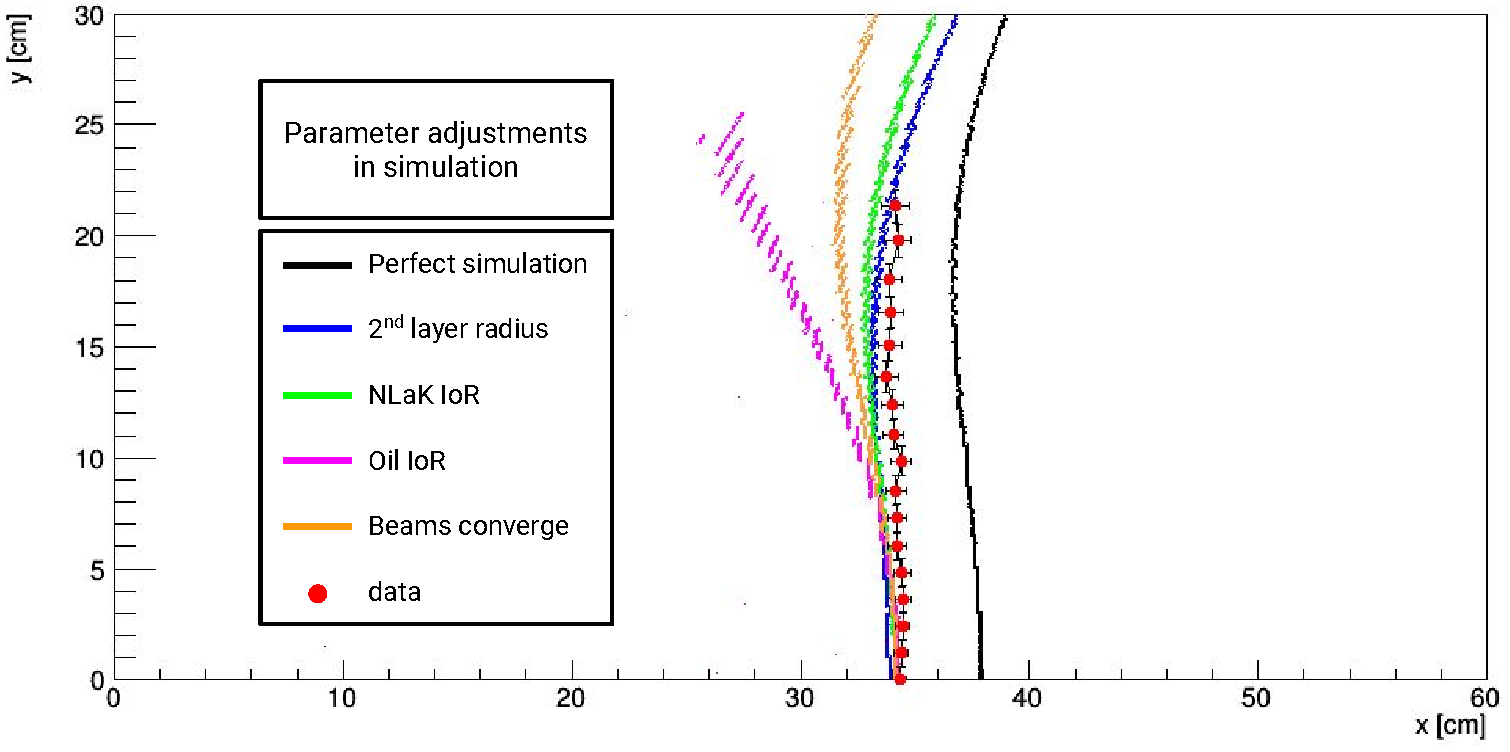
\includegraphics[width=\textwidth]{focal_plane_shifts_together.pdf}
	\caption{Shifting the focal plane of the GEANT4 simulation: decrease the radius of the second layer by $1.3$~mm (blue), increase the refractive index of NLaK33 by $0.03$ (green), decrease the index of refraction of the mineral oil by $0.15$ (pink), and give a converging angle of the laser beams of $0.15$~mrad (black). Experimental data is shown in red and simulation with ``perfect" parameters is shown in black.}
	\label{fig:focal_plane_shifts}
\end{figure}

\begin{figure}[!htb]
	\centering
	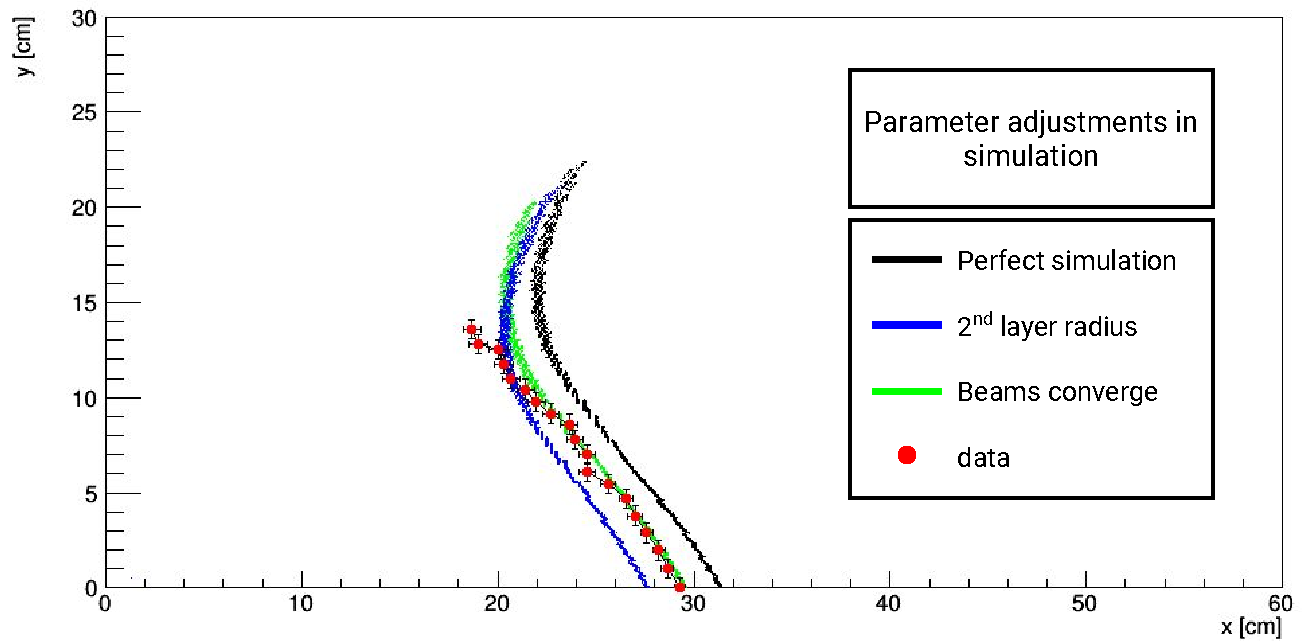
\includegraphics[width=\textwidth]{focal_plane_xshift.pdf}
	\caption{Focal plane after implementing a $7$~mm shift along a line connecting the two beams for data (red) and simulation assuming ``perfect" parameters (black), a reduction in the radius of the second curved surface (blue), and a non-parallelism between the beams (green). Clearly the modification of the radius overcompensates for the change in the position and shape of the focal plane while the non-parallelism assumption agrees very well.}
	\label{fig:focal_plane_xshift}
\end{figure}

%----------------------------------------------------------------------
%	NLAK33 RAD HARDNESS SECTION
%----------------------------------------------------------------------

\clearpage
\section{Radiation Hardness of NLaK33}
Fused silica, which is used for most of the optical components in all current DIRC designs, was already extensively tested in the BaBar and PANDA experiments \cite{RadHardness} and has proven to be radiation hard up to several hundred krad with little to no loss of transmission. The determination of the radiation hardness of NLaK33 is an important study for the EIC R\&D program. 

The irradiation of a pure sample of NLaK33 material was performed at Catholic University of America (CUA) in a Faxitron CP-160 Cabinet X-Radiator System \cite{XRayCabinet} (Figure \ref{fig:x-ray_setup}a). The cabinet allows for a minimum of 6 second X-ray exposure. Photon energy was set to 160 keV with a 6.2 mA current for all exposures of the NLaK33 sample.

A RaySafe ThinX RAD dosimeter \cite{Dosimeter}, shown sitting on the X-ray cabinet shelf in Figure \ref{fig:x-ray_setup}b, was used to measure the radiation dose being delivered to the sample. Unfortunately the exposure time of the dosimeter is limited to less than 10 seconds, so the shortest time setting on the X-ray cabinet was used. This exposure time of 6 seconds was found to be closer to 7.5 seconds by the dosimeter due to rise and fall time of the source. This shortest exposure time consistently gave readings of 81.4 rad. The dosimeter has a circular active area of $706.9\unit{mm}^2$ while the side of the NLaK33 sample that was exposed to the source has an area of $8\times28\unit{mm}^2$, so the dose delivered to the sample is approximately 25 rad.

To measure the transmission of the sample a LAMBDA 950 UV/Vis/NIR Spectrophotometer \cite{Monochromator} (Figure \ref{fig:monochromator_setup}a), referred to from here on as a monochromator, was used. The monochromator has a dynamic range between 175 - 3,300 nm wavelength in 1 nm steps. The sample of NLaK33 was held in place using an optics stand (Figure \ref{fig:monochromator_setup}b) to make sure measurements were consistent and reproducible. Measurements of the transmission of the sample were taken between each set of radiation exposures. The transmission of sample of fused silica was also tested between each radiation exposure of the NLaK33 sample, but was only used as a control sample and was found to be stable.

Because it was not clear exactly what percentage of the total dose read by the dosimeter was from the warm up and cool down of the cabinet it was decided that the best approach for exposure of the sample was to do multiple steps of the 6 second exposure time and record the accumulated dose in this manner. The first exposure was 4 intervals for a total of 100 rad. After this measurement it was noticed that there was already a roughly 2\% drop in the transmission of the sample at 420 nm wavelength \footnote{420~nm wavelength was chosen because it is near the peak of the quantum efficiency of the multi-channel plate photomultiplier tubes discussed later in this chapter and used in the analysis presented in Chapter \ref{ch:analysis}}, so steps of 50 rad were taken for the next several measurements. After 700 rad of dose it was clear that there was a linear correlation between accumulated dose and loss in transmission, so it was decided that 100 rad steps could again be taken. 

Results for the radiation hardness tests of the NLaK33 sample are shown in Figure \ref{fig:transmission_measurements}. The transmission loss below roughly 350~nm wavelength and above 700~nm wavelength seems to be negligible. However, in the range of 350-700~nm there is a clear dip in transmission. At 420~nm wavelength, corresponding to the peak in the quantum efficiency of the photodetectors used in the DIRC, sees a 1.3\% drop in transmission per 50 rad of dose. While it is not yet clear what the expected integrated dose will be in the area of the DIRC at the EIC it is assumed that this loss is too great over the lifetime of the detector. Other materials known to be radiation hard, such as lead fluoride, are being investigated as possible alternatives.

\begin{figure}[!htb]
	\centering
	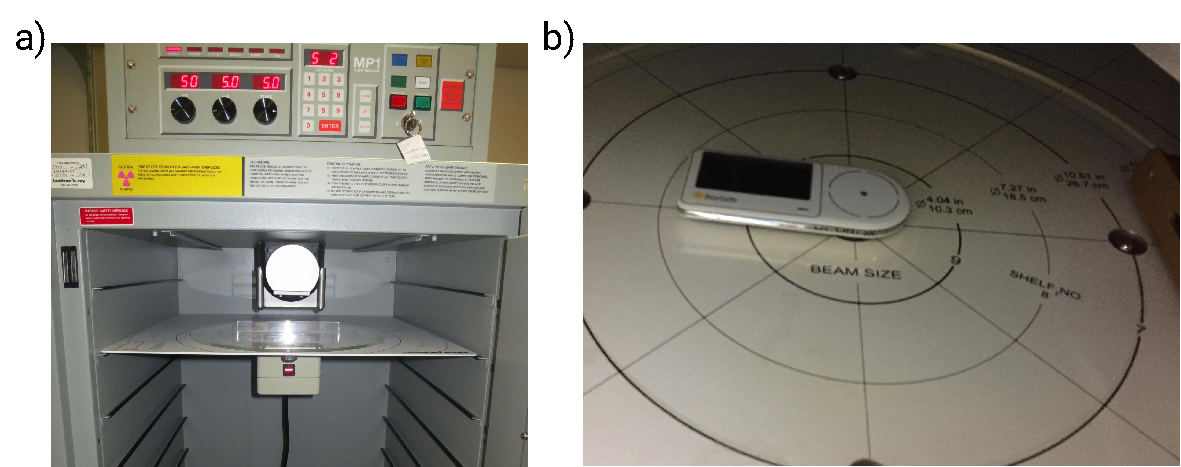
\includegraphics[width=\textwidth]{x-ray_setup.pdf}
	\caption{The Faxitron CP-160 Cabinet X-Radiator System (a) used to irradiate the NLaK33 sample with 160 keV photons at 6.2 mA current for 6 second intervals, and the RaySafe ThinX RAD Dosimeter (b) sitting on one of the X-ray cabinet shelves.}
	\label{fig:x-ray_setup}
\end{figure}


\begin{figure}[!htb]
	\centering
	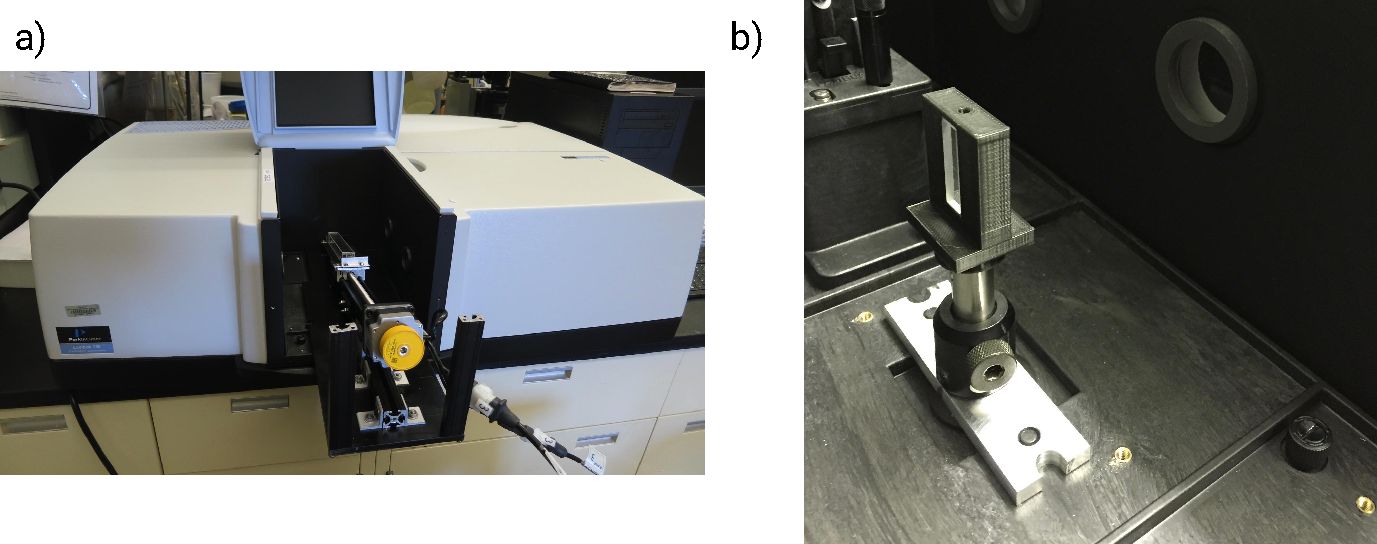
\includegraphics[width=\textwidth]{monochromator_setup.pdf}
	\caption{The LAMBDA 950 UV/Vis/NIR Spectrophotometer (a) and a closeup view of the NLaK33 sample being held in position by the optics stand (b).}
	\label{fig:monochromator_setup}
\end{figure}

\begin{figure}[!htb]
	\centering
	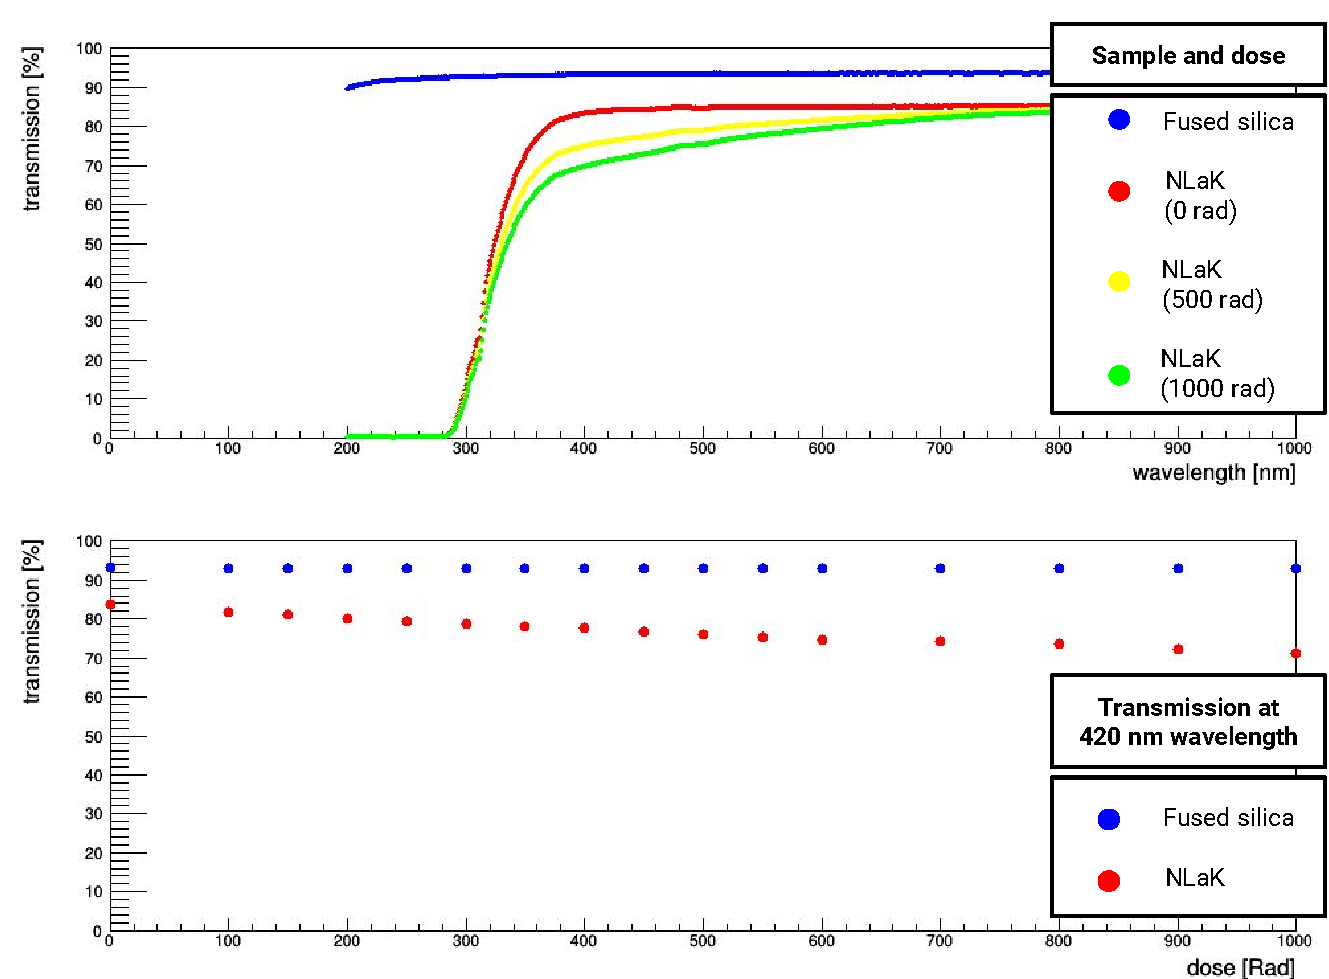
\includegraphics[width=\textwidth]{transmission_measurements2.pdf}
	\caption{The top plot shows the transmission of the control sample of fused silica (blue) and the transmission of the NLaK33 sample after 0 (red), 500 (yellow), and 1000 (green) rad dose across a range of 200-800 nm wavelength. The bottom plot shows the transmission of the NLaK33 sample at 420 nm wavelength as a function of the dosage. After the first 700 rad of dose it was clear that there was a linear relationship between dose and transmission loss, so 100 rad steps were used afterwards.}
	\label{fig:transmission_measurements}
\end{figure}

%----------------------------------------------------------------------

%	HIGH-B TESTS SECTION
%----------------------------------------------------------------------
\clearpage
\section{Performance of MCP-PMTs in High Magnetic Field}
The limiting space requirements of the EIC DIRC design, as mentioned in Chapter \ref{ch:eicdirc}, places a unique set of requirements on the DIRC readout sensors. In order to achieve the desired single photon resolution while maintaining a sufficiently sized expansion volume the sensors, and therefore the pixels, must be compact. Furthermore, due to the positioning of the readout plane inside the large field of the solenoid magnet (see Figure \ref{fig:jleic_layout}) these sensors must also have a high tolerance to magnetic fields, both in magnitude (up to 3 T or higher), non-uniformity, and orientation. Ordinary photomultiplier tubes (PMTs) are not an option due to their susceptibility to magnetic fields, being affected by fields as small as 0.5 Gauss \cite{PMT_magnet}. Silicon photomultipliers (SiPMs) are attractive due to their very compact size and their resistance to magnetic fields up to 4 T \cite{SiPM_characterization}. However, the inherent background, or dark count, of SiPMs is very large, on the order of MHz per pixel \cite{SiPM_characterization} \cite{HamamatsuSiPM}. Because a DIRC detector only expects 100 photons per event at most spread over $100$~ns, this level of background is far too large for usability. The dark noise can be mitigated by cooling, with a decrease by a factor of approximately 2 per $5^\circ$~C, but the large amount of cooling required around the SiPMs in the EIC detector would be costly both in space and finance. With these requirements in mind the best option for an EIC DIRC detector is the use of micro-channel plate photomultiplier tubes (MCP-PMTs) (Figure \ref{fig:MCP_schematic}). The dark count of MCP-PMTs is on the order of kHz \cite{MCPPMT_darkcount}, which is much more acceptable compared to SiPMs. MCP-PMTs also have a much higher resistance to external magnetic fields than traditional PMTs due to the small pore size, with studies being done up to 2 T \cite{MCPTest1}, \cite{MCPTest2}, \cite{MCPTest3}, \cite{MCPTest4}, \cite{MCPTest5}, \cite{MCPTest6}. The tests described below are the first to study the effects of fields as large as 5 T on MCP-PMTs.

\begin{figure}[!htb]
	\centering
	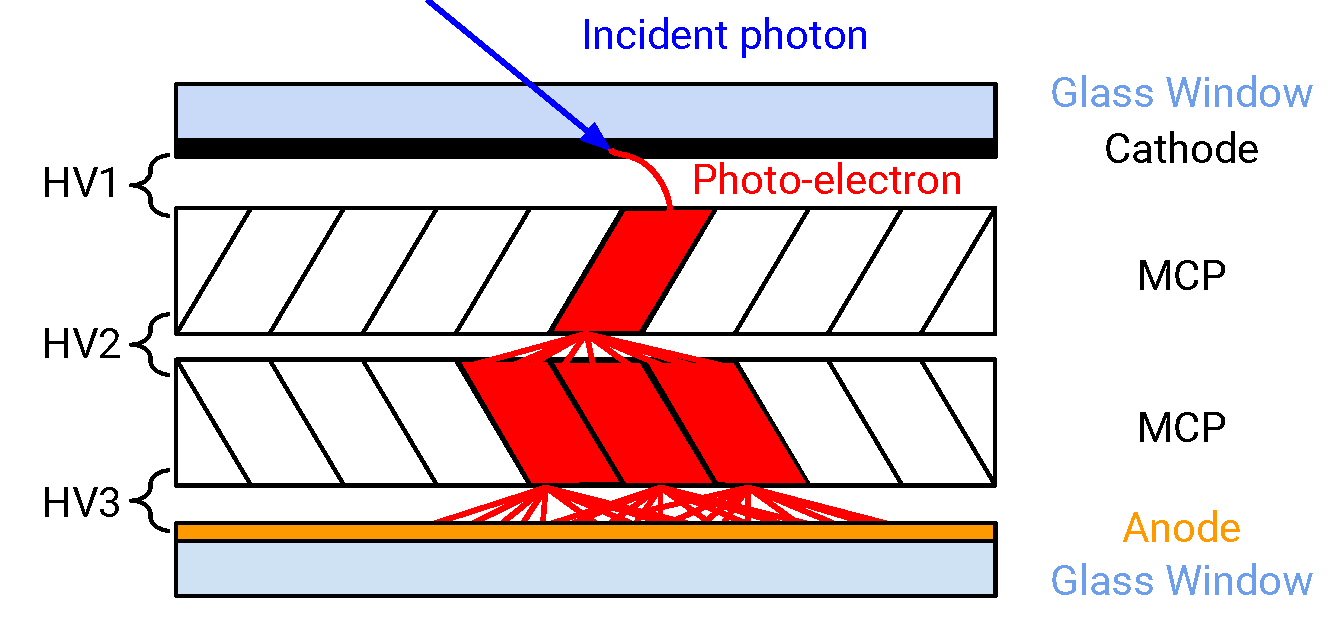
\includegraphics[width=\textwidth]{MCP_schematic.pdf}
	\caption{Schematic of the Micro-channel Plate photo-multiplier tube (MCP-PMT) concept. A cathode and anode sandwich two conducting plates with micrometer-sized channels (MCP), and a high-voltage (HV) difference (HV1, HV2, HV3) between every two components. The channels, or pores, of the two MCPs are aligned in a chevron pattern. An incident photon (blue) strikes the cathode, producing a photo-electron (red). That electron is accelerated through the potential difference between the cathode and first MCP (HV1) before striking the inside of one channel. This creates the same effect as an electron striking the dynode of a typical PMT, resulting in an avalanche of photo-electrons that emerge out of the other side of the first MCP. These electrons are again accelerated through a second potential difference (HV2) before repeating the process in the second MCP. Finally, the copious photo-electrons exit the second MCP, are accelerated through a final potential difference (HV3), and are collected on the anode. This design is both much more compact, more resistant to magnetic fields compared to traditional PMTs, and has less timing jitter. }
	\label{fig:MCP_schematic}
\end{figure}

\subsection{Experimental Setup}
In the fall of 2014 two single-anode MCP-PMTs were tested at Jefferson Lab \cite{HighB_DIRC2015}, a PHOTONIS PP0365G ($6 \mu\text{m}$ pore size and a $18.2 \unit{mm}$ active area) \cite{PHOTONIS} and a Photek PMT210 ($3 \mu\text{m}$ pore size and a $10 \unit{mm}$ active area)  \cite{Photek}, shown in Figure \ref{fig:highB_magnet} at the top and bottom right respectively. The FROST  superconducting solenoidal magnet, with a field tunable up to 5 T with a cylindrical bore diameter of 12.7 cm and a length of 76.2 cm, was used for testing \cite{JLab_FrozenTarget}. The central field of the magnet, while quite large, is also very homogeneous, with an inhomogeneity of less than $5\times10^{-5}$ over a cylindrical volume with a diameter of 1.5 cm and a length of 5 cm. The sensors were held in place at the center of the magnet using a custom-built, non-magnetic, light-tight cylindrical dark box, as shown in Figure \ref{fig:highB_magnet}. Inside the dark box the sensor was held in place by a turn table that allowed for rotation around a vertical axis as well as a horizontal axis (the Y(Y') and Z(Z') axes in Figure \ref{fig:highB_schematics} respectively). The range of the polar angle $\theta$ was dependent on the size of the sensor being measured as well as the signal and HV cables connected to the back of the sensor. A cart allowed the sensor to move relative to the dark box for precise positioning at the center of the magnet. The gain of both sensors were scanned for various angles of $\theta$, $\phi$, and a range of magnetic field from 0 to 5 T.

A pulser-driven LED was used to illuminate the MCP-PMTs with 470 nm photons. An optical fiber was used to transmit the photons to the dark box and a diffuser installed inside the dark box cap was used to illuminate the entire face of the sensor with nearly constant intensity and 10 ns wide pulses at 30 kHz. The sensor signal output was then amplified using a 200-times preamplifier and used as input to a 250~MHz flash analog-to-digital converter (fADC) with 4096 sample depth provided by the JLab Electronics Group. The fADC was then read out by our data acquisition system (DAQ).The pulser was also used as the trigger signal for the fADC, as shown in the chart in Figure \ref{fig:highB_schematics} (right).

My contribution to these studies was assisting in the experimental setup, data monitoring and collection, restructuring and updating the signal reconstruction software, and operating the FROST magnet and electronics both during and between runs. The analysis of the data was done by Dr. Yordanka Ilieva from the University of South Carolina, who's results are shown below and taken, with permission, from \cite{HighB_DIRC2015}.


\begin{figure}[!htb]
	\centering
	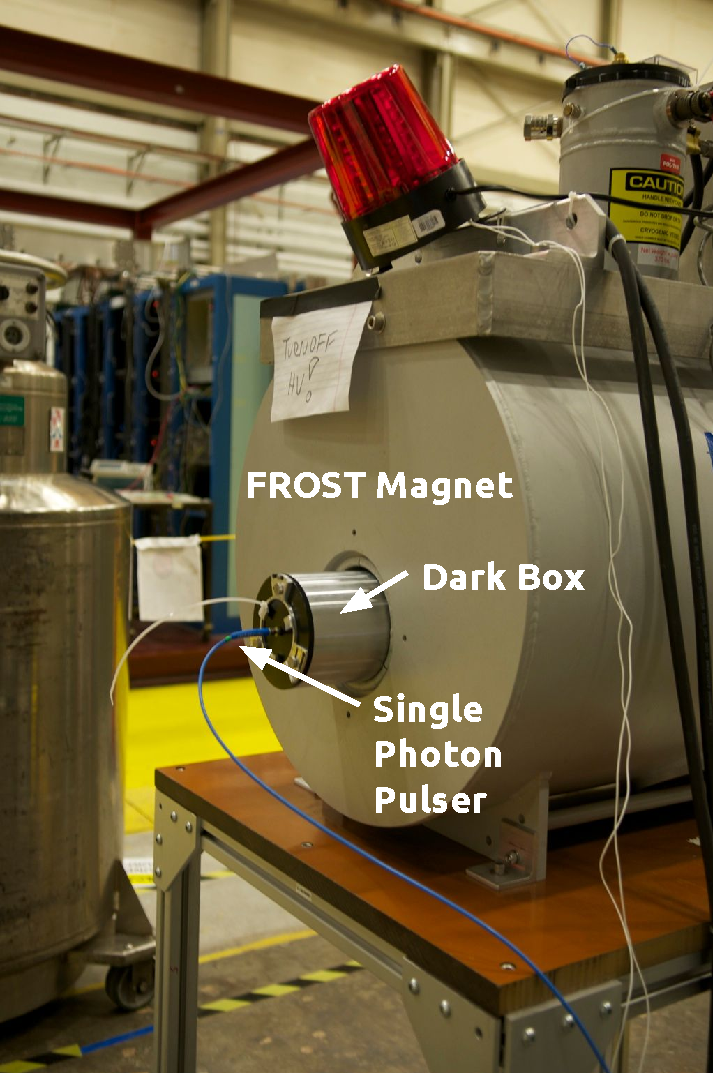
\includegraphics[width=0.8\textwidth]{highB_magnet.pdf}
	\caption{The FROST superconducting magnet (left) with the dark box placed in the bore, and the Photek PMT210 (top right) and PHOTONIS PP0365G (bottom right) MCP-PMTs used for testing at JLab.}
	\label{fig:highB_magnet}
\end{figure}

\begin{figure}[!htb]
	\centering
	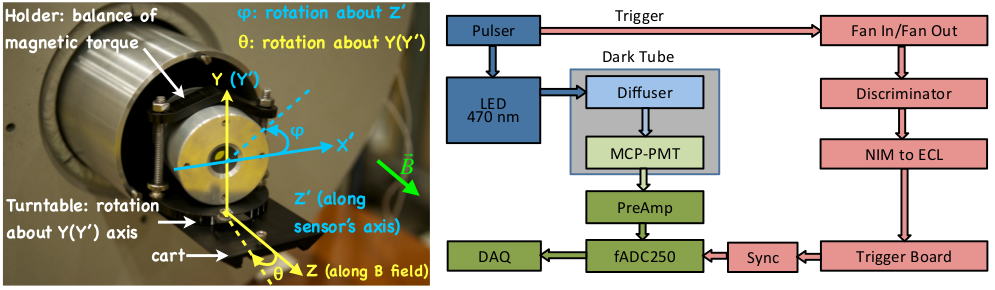
\includegraphics[width=\textwidth]{highB_schematics.png}
	\caption{Left: A closeup of the dark box showing the Photek PMT210 being held in place by the turn table. This setup allows the MCP-PMT to be rotated around both the horizontal Z(Z') axis as well as the vertical Y(Y') axis (with respect to the floor). The rotation about the Y(Y') and Z(Z') axes are described by the polar angle $\theta$ and azimuthal angle $\phi$ respectively. The magnetic field is parallel to the central axis of the dark box. Right: A flowchart of the readout used for testing. The photocathode is exposed to single 470 nm photons to produce photoelectrons, with a large voltage difference between the anode and cathode used to create an avalanche. The total charge is collected on the anode, amplified by a preamplifier, and digitized by an fADC and read out by a DAQ. \cite{HighB_DIRC2015} }
	\label{fig:highB_schematics}
\end{figure}

\subsection{Results}
The gain of the sensors is proportional to the average charge per pulse collected on the sensor anode, and thus the performance can be measured in terms of the average charge collected on the fADC. This is calculated by taking the integral of the fADC signal. The fADC samples the signal every 4 ns in a $1 \mu\text{s}$ window. For each event, $i$, the average pedestal was determined from the fADC using the first 20 bins, and the waveform is integrated over 9 bins around the peak. The integral of the pedestal is subtracted, resulting in a value, $Q_{9,i}$, that is proportional to the total charge collected on the anode for that event. The average values of $Q_{9,i}$ for each setting of field, $\theta$, and $\phi$ are used in the results presented. Figure \ref{fig:highB_waveform} (left) shows an example of a waveform from the PP0365G sensor. Another strategy used for calculating the collected charge was to integrate the entire pedestal-subtracted average waveform (Figure \ref{fig:highB_waveform} right). This yielded results consistent with the event-by-event analysis.

Figure \ref{fig:highB_nominal_HV} shows the performance of both sensors at the nominal ($\theta = \phi = 0^{\circ}$) position for magnetic fields up to 5 T. Data were taken for HV settings of 93\% (black) and 97\% (red) of the maximum manufacturer-recommended HV value. The PP0365G sensor shows a smooth, nearly linear decrease in charge as the field increases, being able to operate at up to 3 T with a factor of 15 loss in collected charge. By increasing the HV the operational range was extended to 3.5 T. The PMT210 has an increase in the collected charge up to 0.5 T with a smooth decrease thereafter as the magnitude of the field increases, staying operational until 4 T with only a factor of 6 decrease in collected charge. Increasing the HV allowed signal to be collected up to 5 T. An uncertainty of 5\%, shown in the error bars of each data point, was the dominant source of error, with the systematic uncertainty giving less of a contribution. The latter was estimated as the standard deviation of the sample of repeated outcomes of the average collected charge at the same setting (mainly the nominal angle setting at a 0 T field) from runs taken randomly throughout the measuring period. The standard deviation acccounts for the variations of the light intensity on the photocathode and of the positioning of the sensor in the dark box.

Figure \ref{fig:highB_QBtheta} shows the response of the sensors at various $\theta$ angles up to $30^{\circ}$. As one can see, the two sensors have very different responses. The magnetic field dependence of the collected charge for the PP0365G shows a maximum below 1 T for $\theta = 20^{\circ}$, $25^{\circ}$, and $30^{\circ}$, while $\theta = 0^{\circ}$ and $10^{\circ}$ show a smooth decrease as magnetic field increases. There is also a much more rapid decrease in collected charge at fields above 1 T for higher angles. The PMT210, however, shows a more uniform characteristic for all $\theta$ angles. For both sensors, as the $\theta$ angle increases the field range in which the sensor can reliably operate becomes more narrow.

The effect of changing the $\phi$ angle of the PP0365G sensor for different magnetic field strengths and $\theta$ angles of $10^{\circ}$ and $20^{\circ}$ can be seen in Figure \ref{fig:highB_QBphi}. Because the outer casing of the sensor is cylindrical and there is no apparent orientation, a $\phi = 0^{\circ}$ position was chosen randomly and marked on the front of the casing for consistency. The rotation was done counterclockwise about the sensor's axis when looking from the front. The data shows that at a fixed $\theta$ angle the collected charge has a $\phi$ dependence, and this dependence is strongly correlated to the $\theta$ angle. The larger $\theta$ angle shows a much faster decrease in collected charge as the $\phi$ angle increases.

\begin{figure}[!htb]
	\centering
	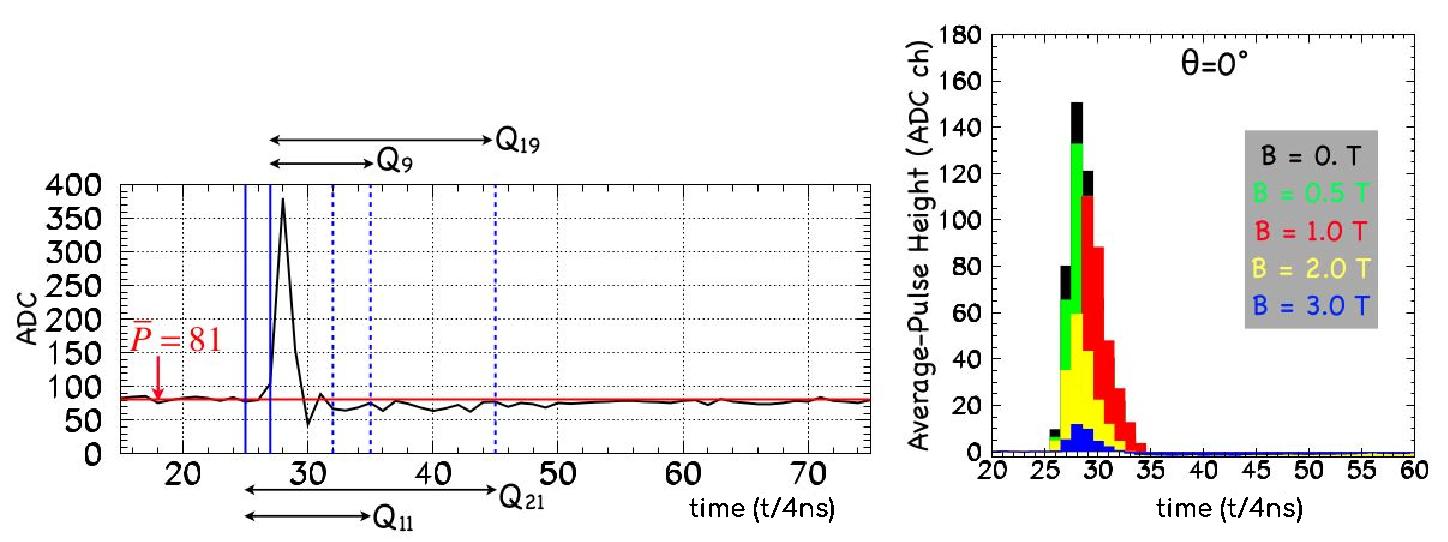
\includegraphics[width=\textwidth]{highB_ADCintegration.pdf}
	\caption{\textbf{Left}: an example waveform measured for the PP0365G sensor. Each bin of the x-axis corresponds to a 4 ns interval. The y-axis is the fADC value (ranging from 0 to 4096). The solid red line shows the calculated pedestal position for the event. The ranges $Q_9$, $Q_{11}$, $Q_{19}$, and $Q_{21}$ denote the positions of integration ranges over 9, 11, 19, and 21 bins respectively for calculation of the total anode charge for that event. The limits and width of the integration range were varied for systematic purposes. \textbf{Right}: the average waveforms of the PP0365G sensor at $\theta = 0^{\circ}$ and varying magnetic field strengths. There is a clear negative correlation between the signal amplitude and field magnitude.}
	\label{fig:highB_waveform}
\end{figure}

\begin{figure}[!htb]
	\centering
	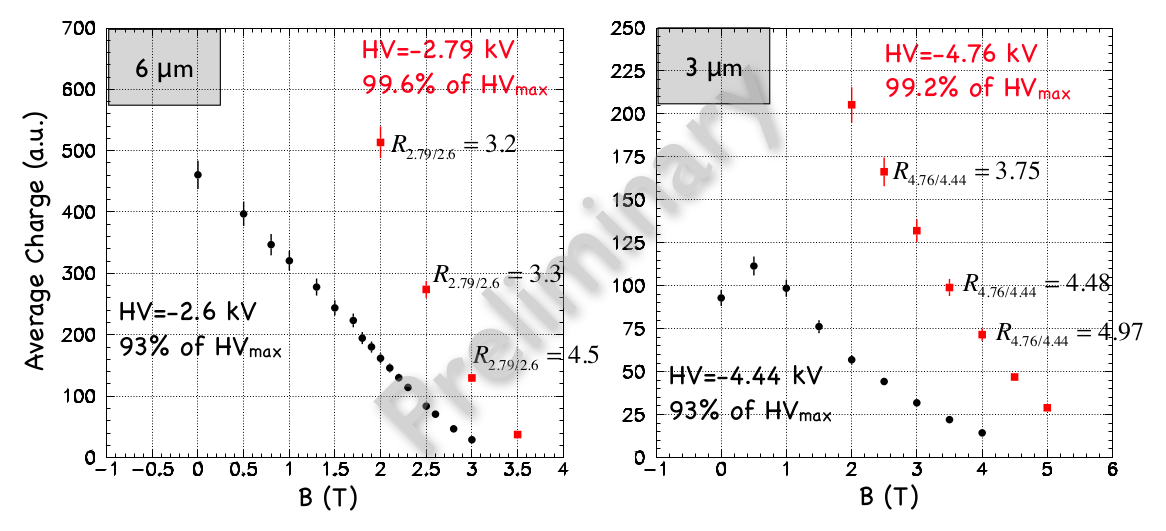
\includegraphics[width=\textwidth]{highB_QBV.png}
	\caption{The gain performance of the PP0365G and PMT210 sensors (left and right) at $\theta = 0^{\circ}$ and two HV settings. The black and red points were measured using 93\% and 99\% of the maximum manufacturer recommended HV (HV\textsubscript{max}) settings respectively. For the PP0365G at 93\% (95\%) of HV\textsubscript{max} a reasonable signal can be obtained up to a 3 (3.5) T field, though the total collected charge decreased by a factor of 15 when going from 0 T to 3 T. The PMT210 was able to produce a signal at fields up to 4 (5) T, and the collected anode charge decreased only by a factor of 6 when going from 0 to 4 T. The error bars on all points include both statistical and 5\% systematic uncertainties, with the latter being the dominate contribution.}
	\label{fig:highB_nominal_HV}
\end{figure}

\begin{figure}[!htb]
	\centering
	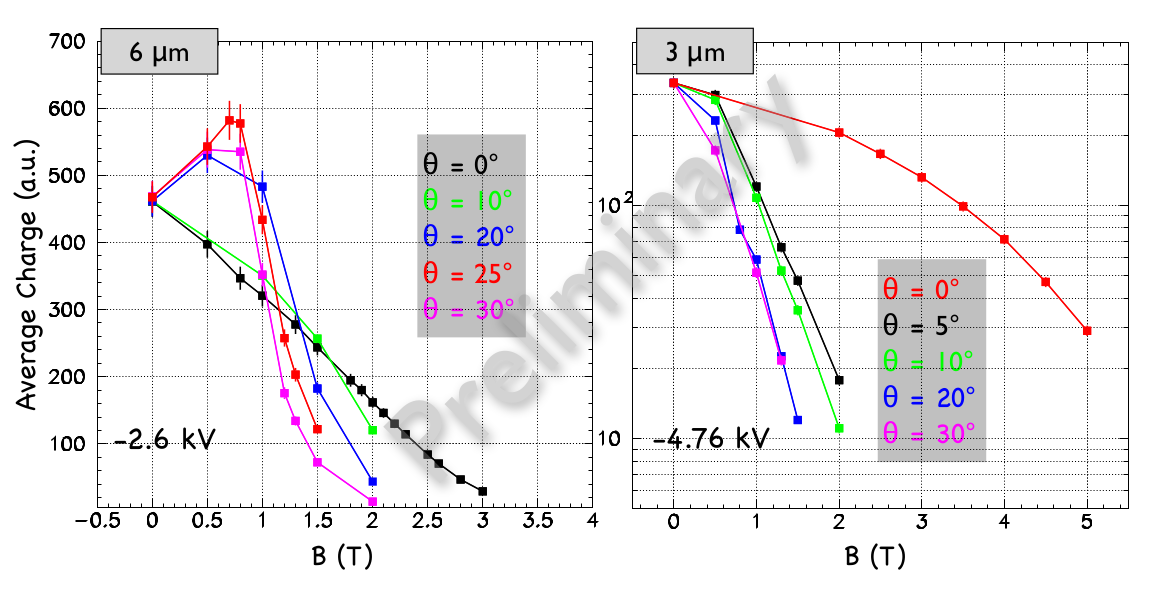
\includegraphics[width=\textwidth]{highB_QBtheta.png}
	\caption{The average collected anode charge as a function of magnetic field strength at various $\theta$ rotation angles for the PPP0365G (left) and PMT210 (right) sensors.}
	\label{fig:highB_QBtheta}
\end{figure}

\begin{figure}[!htb]
	\centering
	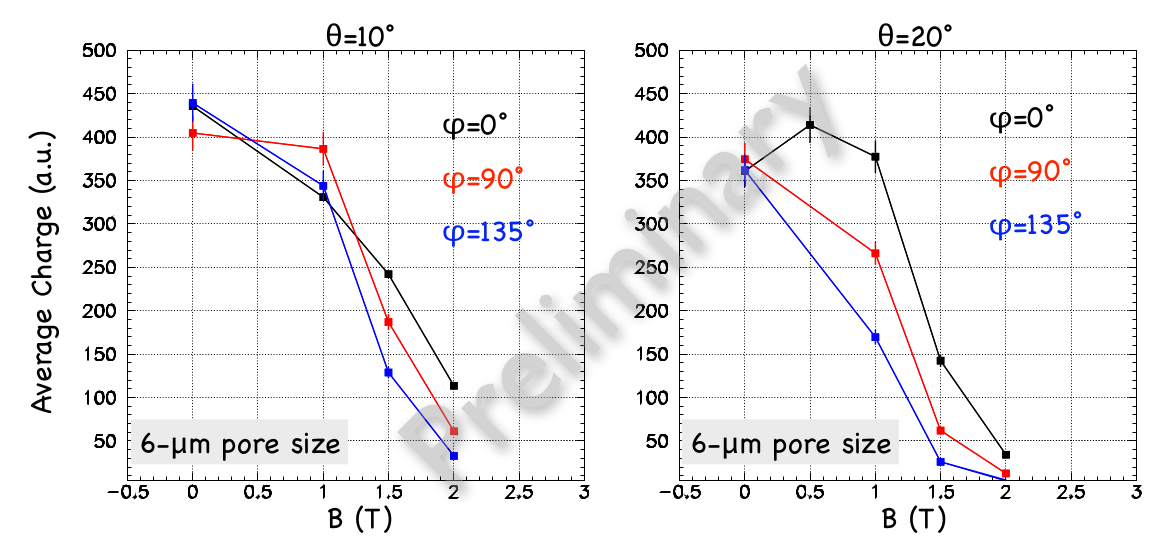
\includegraphics[width=\textwidth]{highB_QBphi.png}
	\caption{The average collected anode charge as a function of magnetic field strength at various $\phi$ rotation angles for the PP0365G at fixed $\theta$ angles of $10^\circ$ (left) and $20^\circ$ (right).}
	\label{fig:highB_QBphi}
\end{figure}

\subsection{Conclusions}
Overall the data at $\theta = 0^{\circ}$ suggests that a smaller pore-size sensor (PMT210) has a higher resistance to the effects of high magnetic fields as it was able to operate up to 5 T fields and had a slower decrease in collected charge with increasing field than the PP0365G sensor. The smaller pore-size sensor as showed an higher increase in collected charge with increased HV. When increasing the $\theta$ angle, however, the PMT210 showed a much more rapid decrease in performance compared to the PP0365G. At $0^{\circ}$ the PMT210 can be operated up to 5 T, while rotating to $5^{\circ}$ there is a dramatic decrease in maximum field to 2 T. The PP0365G sensor, however, was more stable with rotations in $\theta$, dropping from 3 T at $0^{\circ}$ to 2 T at larger angles.

While the data for the two sensors allow to make general conclusions about the effect of pore size on performance, more detailed conclusions cannot be made with certainty as the orientation of the MCPs inside the sensors are not necessarily the same. While the definition of the $\theta$ angle is consistent for both sensors in this testing, the azimuthal orientation of the channels relative to the central axis may differ greatly. No details are given by the manufacturer about the absolute azimuthal orientation of the channels for each sensor as this information has not as of yet been necessary for applications of MCP-PMTs. These data, however, suggest that this will be important for optimization of the sensor design and operational parameters for operations in areas of non-homogeneous, high-strength magnetic fields, such as for the EIC DIRC.
